\documentclass[../monografia.tex]{subfiles}
\graphicspath{ {images/}{../images/} } 

\begin{document}
% Detalhar neste item os procedimentos realizados para os testes de funcionamento dos sub-sistemas, da inter-relação dos subsistemas e do sistema completo.

\section{Resultados dos Testes}
\section{Verificação dos requisitos}

\begin{figure}[h!]
	\centering
	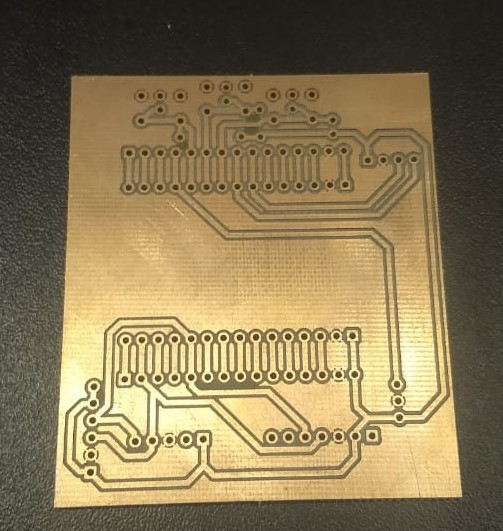
\includegraphics[width=10cm]{pcb-fresada}
	\caption{PCB fresada}
	\label{fig:img5}
	\end{figure}
	
%? Montagem final da placa

\begin{figure}[h]
	\centering
	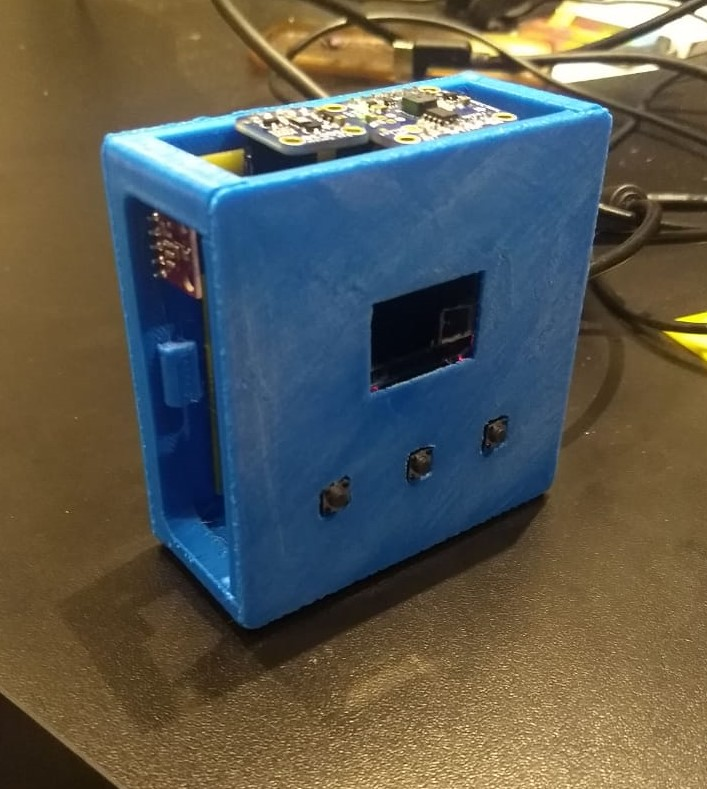
\includegraphics[width=0.8\textwidth]{montagem-final.jpg}
	\caption{Montagem final do protótipo}
	\label{fig:prototipo}
\end{figure}

\end{document}